\documentclass[a4paper, 12pt, final, garamond]{book}
\usepackage{cours-preambule}

\raggedbottom

\makeatletter
\renewcommand{\@chapapp}{Programme de kh\^olle -- semaine}
\makeatother

\begin{document}
\setcounter{chapter}{15}

\chapter{Du 23 au 27 janvier}

\section{Cours et exercices}
\section*{Mécanique chapitre 1 -- Cinématique du point}
\begin{enumerate}[label=\Roman*]
    \item \textbf{Système et point matériel}~: définition système, point
        matériel.
    \item \textbf{Description et paramétrage du mouvement}~: notion de
        référentiel, relativité du mouvement, exemples de référentiels, vecteur
        base de projection et repère.
    \item \textbf{Position, vitesse et accélération}~: position et déplacement
        élémentaire, équations horaires et trajectoires~; vitesse et vitesse
        instantanée, notation pointée~; accélération et accélération
        instantanée.
    \item \textbf{Exemples de mouvements}~: rectiligne uniforme, rectiligne
        uniformément accéléré, courbe uniformément accéléré.
\end{enumerate}

\section*{Mécanique chapitre 2 -- Dynamique du point}
\begin{enumerate}[label=\Roman*]
    \item \textbf{Introduction}~: inertie et quantité de mouvement, forces
        fondamentales.
    \item \textbf{Trois lois de \textsc{Newton}}~: principe d'inertie, principe
        fondamental de la mécanique, loi des actions réciproques.
    \item \textbf{Systèmes de points}~: centre d'inertie, quantité de mouvement
        d'un ensemble de points, théorème de la résultante cinétique.
    \item \textbf{Méthode générale de résolution}.
    \item \textbf{Le poids}~: définition, chute libre avec angle initial.
    \item \textbf{Poussée d'\textsc{Archimède}}.
    \item \textbf{Frottement fluide}~: force de frottement fluide, chute libre
        sans vitesse initiale avec frottements linéaires, avec frottements
        quadratique, résolution par adimensionnement.
    \item \textbf{Frottements solides}~: réaction, lois de \textsc{Coulomb}.
    \item \textbf{Tension d'un fil}
    \item \textbf{Force de rappel d'un ressort}~: force de rappel élastique,
        position d'équilibre verticale.
\end{enumerate}

\section{Cours uniquement}
\section*{Mécanique chapitre 3 -- Mécanique des mouvements courbes}
\begin{enumerate}[label=\Roman*]
    \item \textbf{Mouvement courbe dans le plan}~: position, vitesse,
        déplacement élémentaire, accélération en coordonnées polaires.
    \item \textbf{Exemples de mouvements plans}~: mouvement circulaire,
        circulaire uniforme, repère de \textsc{Frenet}.
    \item \textbf{Application~: pendule simple}
    \item \textbf{Mouvement courbe dans l'espace}~: coordonnées cylindriques,
        coordonnées sphériques.
\end{enumerate}

\section{Questions de cours possibles}
\begin{enumerate}[label=\sqenumi]
    \item Présenter les coordonnées cylindriques avec un schéma introduisant la
        base et indiquant les coordonnées, donner l'expression de $\OM$ dans
        cette base, donner \textbf{et démontrer} l'expression de la vitesse, du
        déplacement élémentaire et de l'accélération en coordonnées cylindriques.
    \item Présenter succinctement la base de \textsc{Frenet} sur une trajectoire
        quelconque (cercle osculateur), écrire les vecteurs vitesse et
        accélération dans cette base en fonction de $v$, $R$ et $\dot{v}$.
    \item Présenter les coordonnées sphériques et donner le déplacement
        élémentaire.
    \item Énoncer les trois lois de \textsc{Newton}, définir le centre d'inertie
        d'un ensemble de points, le vecteur quantité de mouvement d'un
        ensemble de points et son lien avec le centre d'inertie, énoncer et
        démontrer le théorème de la résultante cinétique.
    \item Déterminer les équations horaires du mouvement rectiligne uniformément
        accéléré. Une attention particulière sera portée à l'établissement du
        système d'étude.
    \item Déterminer les \textbf{équations horaires} ainsi que la
        \textbf{trajectoire} du lancer d'une masse avec une vitesse initiale
        $\vf_0$ faisant un angle $\alpha$ avec l'horizontale. Une attention
        particulière sera portée à l'établissement du système d'étude.
        Déterminer alors la portée, la flèche du tir ainsi que le temps de vol,
        au choix (potentiellement multiple) de l'interrogataire.
    \item Déterminer la vitesse limite et le temps caractéristique du mouvement
        pour une chute libre sans vitesse initiale avec frottements linéaires.
        Les approches d'adimensionnement d'équation différentielle, de solution
        limite ou de résolution totale sont possibles.
    \item Présenter les lois du frottement de \textsc{Coulomb}, et refaire
        l'exercice~:
\end{enumerate}
\begin{NCexem}[width=\linewidth]{Plan incliné et frottements solides}
    \begin{minipage}{0.6\linewidth}
        On considère un plan incliné d'un angle $\alpha = \ang{20;;}$ par
        rapport à l'horizontale. Une brique de masse $m = \SI{600}{g}$ est
        lancée depuis le bas du plan vers le haut, avec une vitesse $v_0 =
        \SI{2.4}{m.s^{-1}}$. Pour étudier le mouvement, on utilise le repère
        (O,$x$,$y$) avec O coïncidant avec la position de départ de la brique.
        On note $g$ l'accélération de la pesanteur, avec $g =
        \SI{9.81}{m.s^{-2}}$. On suppose qu'il existe des frottements solides,
        avec $f$ le coefficient de frottements solides tel que $f =
        \num{0.20}$.\bigbreak
    \end{minipage}
    \hfill
    \begin{minipage}{0.35\linewidth}
        \begin{center}
            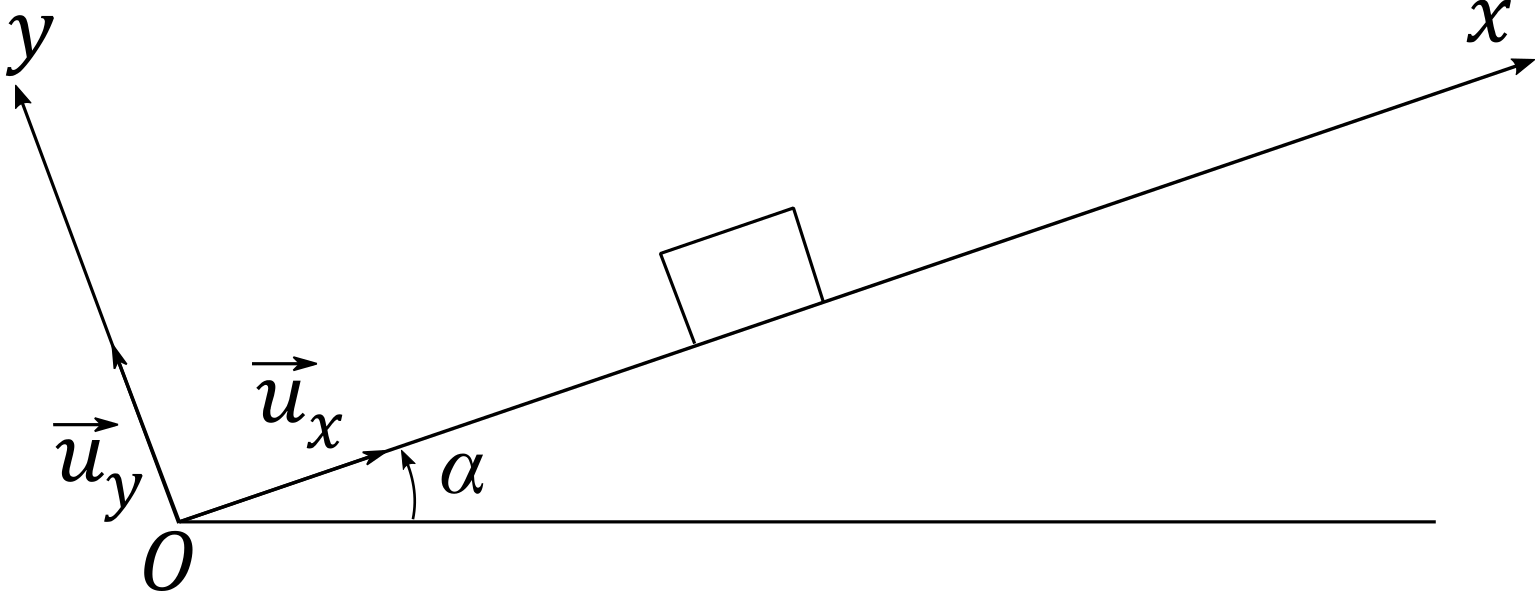
\includegraphics[width=\linewidth]{plan_incl-plain}
        \end{center}
    \end{minipage}
    \begin{enumerate}
        \item Établir l'équation horaire du mouvement de la brique lors de
            sa montée.
        \item Déterminer la date à laquelle la brique s'arrête, ainsi que la
            distance qu'elle aura parcourue.
    \end{enumerate}
\end{NCexem}
\begin{enumerate}[label=\sqenumi, resume]
    \item Étude du pendule simple~: mise en situation, équation différentielle,
        linéarisation, résolution.
    \item Position d'équilibre d'un ressort vertical~: présenter le système,
        déterminer l'équation différentielle sur la position de la masse,
        déterminer la longueur d'équilibre, solution pour des conditions
        initiales données par l'interrogataire.
\end{enumerate}

\end{document}
